%!TEX root = Main.tex

\vsp
\subsection{\auspice\ vs. managed DNS providers}
\label{sec:managed}
%In DNS terminology, an \auspice\ name server provides the functionality of an authoritative name server -- it keeps the most up to date  name-to-address mapping of a host.
 

Can demand-aware replication benefit commercial managed DNS providers that largely rely on statically replicating today's (hardly mobile) domain names? To investigate this, we compare \auspice\ against three top-tier providers, UltraDNS, DynDNS, and DNSMadeEasy %\cite{ultradns, dyndns, dnsmadeeasy}, 
that offer geo-replicated authoritative DNS services widely used by enterprises (e.g., Dyn provides DNS service for Twitter).


%Having analyzed a synthetic workload dominated by mobile device names, we next evaluate how \auspice\ compares to commercial managed DNS providers in serving their customers' (mostly static) domain names.  These providers such as UltraDNS, DynDNS, and DNSMadeEasy \cite{ultradns, dyndns, dnsmadeeasy} offer a geo-replicated authoritative DNS service and are widely used by enterprises today (e.g., DynDNS provides DNS service for Twitter).

%Similar to the role of a replica of a name record in \auspice, managed DNS providers such as UltraDNS, DynDNS, and DNSMadeEasy \cite{ultradns, dyndns, dnsmadeeasy}  offer a geo-replicated authoritative DNS service for domain names.%\footnote{DNS Services such as Open DNS \cite{opendns}, and Google DNS \cite{googledns} maintain local name servers that store cached name records  and therefore are not managed DNS services.}

%Note that Open DNS \cite{opendns}, Google DNS \cite{googledns} and other similar services which offer name lookup service to their users  maintain local name servers that store cached name records  and therefore are not managed DNS services. 


%Managed DNS providers such as UltraDNS, DynDNS, and DNSMadeEasy \cite{ultradns, dyndns, dnsmadeeasy} offer a geo-replicated authoritative DNS service similar to \auspice.
%Managed DNS providers differ from services such as Open DNS \cite{opendns}  and Google DNS \cite{googledns} as the former maintain authoritative name servers for domain names of their customers and the latter maintain local name servers that store cached name records. 



%Managed DNS providers \cite{ultradns,dyndns,dnsmadeeasy} offer a geo-replicated DNS service, and are commonly purchased by enterprises today. This Section \compares \auspice\ to managed DNS providers in terms of lookup and update latencies. 

\subsubsection{Lookup latency}  


We compare \auspice\ to UltraDNS for a workload of lookups for  domain names serviced by the provider. We identify 316 domain names among the top 10K Alexa websites serviced by this provider, and determine
the geo-distribution of lookups for each name from their data \cite{alexa}.
For each name, we measure the latency for 1000 lookups from across 100 PlanetLab nodes. 
We ensure that lookups are served from the name servers maintained by the provider by requesting the address for a new random sub-domain name each time, e.g, \verb+xqf4p.google.com+ instead of \verb+google.com+, that is unlikely to exist in a cache and requires an authoritative lookup.
\auspice\ name servers are deployed across a total of 80 PlanetLab locations while UltraDNS has 16 known server locations \cite{dnscompare}.  
We evaluate \auspice\ for three configurations  with 5, 10, and 15 replicas of a name respectively. 

%For an even comparison between \auspice\ and the provider, we limit the maximum number of replicas/name for \auspice\ to 5, which is less than one-third the number of locations of the provider \cite{dnscompare}.  
%The geo-distribution of lookups for each domain name is determined based on the Alexa dataset \cite{alexa}.




%The list of MDNS deployments is obtained from this report \cite{dnscompare}. The median and maximum different between \auspice\ name server and the corresponding MDNS deployment was X miles and Y miles respectively.  



%\begin{figure}[t]
%\centering
%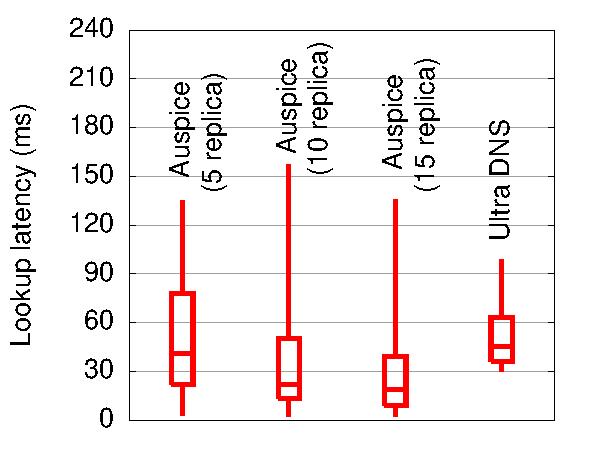
\includegraphics[scale=0.6]{graph/camera-ready/managed-lookup.pdf}
%\vspace{-0.2in}
%\caption{\auspice\ gives better cost-performance tradeoffs than UltraDNS. \auspice\ with 5 replicas has comparable latency to UltraDNS (16 replicas); \auspice\ with 15 replicas has 60\% lower lookup latencies than UltraDNS. Box plot shows 5, 25, 50, 75, and 95 percentiles.}
%\label{fig:managed-lookup}
%\end{figure}

\blue{
Figure \ref{fig:managed-lookup} shows the lookup latencies of names for \auspice\ and for UltraDNS.
UltraDNS incurs a median latency of 45 ms with 16 replicas,  while \auspice\ incurs  41 ms, 22 ms, and 18 ms  respectively with 5, 10, and 15 replicas. 
With 5 replicas, \auspice's performance is comparable to UltraDNS with one-third  the replication cost. 
With 15 replicas, \auspice\ incurs 60\% lower latency for a comparable cost. The comparison against the other two, Dyn and DNSMadeEasy, is qualitatively similar \cite{techreport}.
Thus, \auspice's demand-aware replication achieves a better cost--performance tradeoff compared to static replication.
}




\subsubsection{Update propagation delay} 
To measure update propagation delays, we purchase DNS service from three providers for separate domain names.  All providers replicate a name at 5 locations across US and Europe for the services we purchased. We issue address updates for the domain name serviced by that provider and then immediately start lookups to the authoritative name servers for our domain name.
These authoritative name servers can be queried only via an anycast IP address, i.e., servers at different locations advertise the same externally visible IP address. Therefore, to maximize the number of provider locations queried, we send queries from 50 random PlanetLab nodes. From each location, we periodically send queries until all authoritative name server replicas return the updated address.  The update propagation latency at a node is the time between when the node starts sending lookup to when it receives the updated address. The latency of an update is the the maximum update latency measured at any of the nodes. We measure latency of 100 updates for each provider.
 %is time difference between when we update an address and when the node gets the updated address. 

To measure update latencies for \auspice, we replicate 1000 names at a fixed number of PlanetLab nodes across US and Europe. The number of nodes is chosen to be 5, 10, and 20 across three experiments. A client sends an update to the nearest node and waits for update confirmation messages from all replicas. The latency of an update is the time difference between when the client sent an update and when it received the update confirmation message from all replicas (an upper bound on the update propagation delay).  We show the distribution of measured update latencies for \auspice\ and for three managed DNS providers in Figure \ref{fig:manageddnsupdate}.   

\auspice\ incurs lower update propagation latencies than all three providers for an equal or greater number of replica locations for names. We were unable to ascertain from UltraDNS why their update latencies are an order of magnitude higher than network propagation delays, but this finding is consistent with a recent study \cite{dnscompare} that has shown latencies of up to tens of seconds for these providers. Indeed, some providers even distinguish themselves by advertising shorter update propagation delays than competitors \cite{dnscompare}.

\vspace{-0.1in}
{\paragraph{Sensitivity analyses and other results}} \label{sec:other} We have conducted a comprehensive evaluation of the sensitivity of \auspice's performance-cost trade-offs to workload and system parameters across scales varying by several orders of magnitude. These include workload parameters such as geo-locality, read-to-write rate ratio, ratio of device-to-service names, etc. and system parameters such as the fault-tolerance threshold, capacity utilization, perturbation knob, the tunable overhead of replica reconfiguration, etc. using a combination of simulation and system experiments. These results do not qualitatively change the findings in this paper, and are deferred to the technical report \cite{techreport}.

%To assess the sensitivity of \auspice's benefits to a broad range of system and workload parameters and scales, we develop a custom simulator that simulates round-trip delays, loss, and server load-vs-response time behavior, and have verified \cite{techreport} that the median latencies for all simulated schemes are within 8\% of those in Section \ref{sec:comparison}. We present one such experiment here, deferring others to a technical report \cite{techreport}.

%Figure \ref{fig:varylocality} compares the latency for workloads with varying  geo-locality. Both \staticthree\ and \codons\ are choose replica locations randomly, and therefore their latency remains the same irrespective of the workload's geo-locality. But \auspice\ significantly improves latencies  as the geo-locality increases. Even in a workload with no locality ($g$=0.1),   \auspice\ outperforms \staticthree\ by 2$\times$ because it creates more than three replicas for each name,  and outperforms \codons\ by $4\times$  because it redirects requests to the closest replica of a name without DHT routing.

%Other experiments evaluating the sensitivity of \auspice's performance-cost trade-offs at different scales to workload parameters such as the ratio of device-to-service names, overall lookup-to-update ratio, and system parameters such as the fault-tolerance, capacity utilization, and reconfiguration epoch length are deferred to the technical report \cite{techreport}.

\rmCR{
\subsection{Simulation-based sensitivity analysis}
\label{sec:sensitivity}

In order to assess the sensitivity of \auspice's performance and cost to a wider range of system parameters, workload parameters in Section \ref{sec:comparison}, and scales, we use a custom simulator that simulates round-trip delays, loss, and server load-vs-response time behavior as in the PlanetLab experimental setup. We have verified \cite{techreport} that the median latencies for all simulated schemes are within 8\% of those in the emulation in Section \ref{sec:comparison}.   Experiments here use 10K name servers, 2K local name servers, 10K service names, and 100K device names. 

%We analyze the sensitivity of \auspice's benefits to the workload parameters used in Section \ref{sec:comparison}. In order to be able to explore a wider range of parameters and scales, we use a custom simulator that simulates round-trip latency, loss, and server load-vs-response time behavior as measured on PlanetLab. We have verified \cite{techreport} that the median latencies for all schemes in the simulator are within 8\% of that on PlanetLab for the experiment in Section \ref{sec:comparison}.   Experiments here use 10K nameservers, 2K local nameservers, 10K service names, and 100K device names. 

\textbf{Geo-locality.}  Figure \ref{fig:varylocality} compares the latency for workloads with varying levels of geo-locality.
Both \staticthree\ and \codons\ are choose replica locations randomly, and therefore their latency remains the same irrespective of the workload's geo-locality. But \auspice\ significantly improves latencies  as the geo-locality increases. Even in a workload with no locality ($g$=0.1),   \auspice\ outperforms \staticthree\ by 2$\times$ because it creates more than three replicas for each name,  and outperforms \codons\ by $4\times$  because it redirects requests to the closest replica of a name without the overhead of DHT routing.

\textbf{Ratio of device-to-service names.} We also evaluate schemes for workloads with different ratios of device names to service names. We fix the number of service names to be 10K and vary the number of device names between 1000 to 1M.
%\replicateall\  saturates server capacity for a workload with  DS-ratio = 1 due to high update costs. 
For the given capacity, \auspice\  can accommodate a workload with up 1M device names (while \replicateall\ can support at most 1K device names) and provides up to 6.9$\times$ lower latencies over \staticthree\  across for all ratios of service-to-device names.

% up to 100  as it minimizes the update cost for device names. 
% \auspice\ has up to 6.9$\times$ lower latency than \staticthree\ and \codons\ due to itts locality-aware design,

\textbf{Lookup-to-update ratio.} We vary the ratio of lookups to updates, termed as \emph{RW-ratio}, by increasing the number of lookups but keeping the number of updates fixed. \auspice\ provides up to 2.95$\times$ lower latencies than \codons\ and \staticthree\ for both write-dominated workload (RW-ratio $<$ 1) as well as read-dominated workloads (RW-ratio  $>$ 1). As RW-ratios increase beyond 1,  \auspice\ handles the increase in number of lookups  by automatically decreasing the replication parameter $\beta$ (refer to Eq. \ref{eq:mu}).

\blue{
\textbf{System parameters.} We also experiment with the system parameters in Section \ref{sec:design}, the fault tolerance threshold $F$, the capacity utilization $\mu$, and the randomness knob $\nu$. As expected, we find that as $F$ increases and approaches the total number of name servers, the cost and performance behavior increasingly mimics \static{F} until it is identical to \replicateall. Decreasing $\mu$ to small values makes \auspice's replication less aggressive hurting performance but reducing cost, while increasing $\mu$ much closer to 1 hurts latencies by overloading the system. The technical report \cite{techreport} describes these results as well as a slightly modified replica placement strategy that makes the random perturbation knob $\nu$ unnecessary (currently manually set to 0.5 in our experiments).
}
}


%\textbf{Lookup rate distribution:} We evaluate performance for (a) Zipf  and (b) uniform popularity distribution of  lookup rates of users The mean lookup rates are same for both distributions. As Figure \ref{fig:lookupdis} shows, the lookup latency of all schemes are nearly equal for the two distributions.  The performance of \staticthree\ is unchanged because its replica placement is fixed. \codons\ sees high latency for both distributions because its design replicates most names at a small number of locations for both distributions (a small percent of highly popular names are replicated at larger number of locations). The median lookup rates are smaller for Zipf-distribution compared to uniform distribution, i.e., a typical name has a smaller read-to-write ratio for Zipf-distritbution compared to uniform distribution . Hence, \auspice\ create less number of replicas for most names. Still, the number of replicas for names is sufficiently high in this experiment to keep the lookup latency nearly the same. 

%The slightly better latencies for \auspice\ for the Zipf-distribtuion are because of  highly popularity names see a improv

%\codons\ decides number of replicas only based on popularity ranking of a name and not on the value of the lookup rates, and hence its distribution of the number of replicas of names remains unchanged due to a change in the popularity distribution. 

%The performance of \codons\ and \staticthree\ are unchanged as they 

%Across experiments, we change the distribution of lookup rates of users keeping the average lookup rate unchanged.  Figure X shows the results. 

%This experiment suggests that our results from prior experiments are likely to hold irrespective of the specific distribution of lookup rates of users.


\eat{
\begin{figure}
\centering
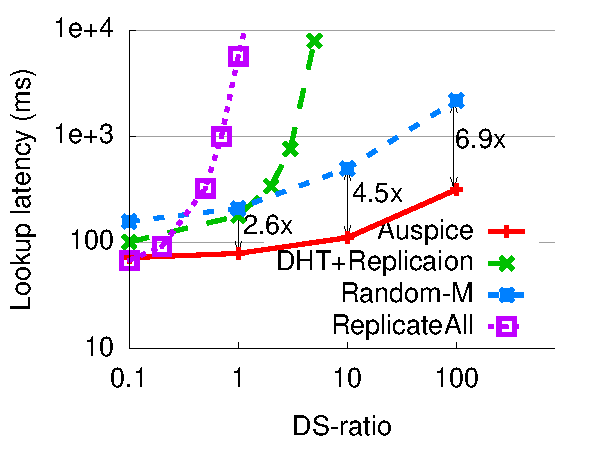
\includegraphics[scale=0.5]{graph/medianlatencyVSnummobile.pdf}
\vspace{-0.1in}
\caption{[Simulator] \auspice\ gives greater latency gains over \staticthree\ as the number of device names increases in  the workload.}
\label{fig:varymobile}
\end{figure}

\textbf{Ratio of device names to service names:} This experiment evaluates schemes for workloads with different ratios of device names to service names, called \emph{DS-ratio} for short.
We fix the number of service names to be 10K and vary the number of device names between 1000 to 1,000,000.
Figure \ref{fig:varymobile} presents our results.
\replicateall\  saturates server capacity for a workload with  DS-ratio = 1 due to high update costs. 
\auspice\  supports workloads with DS-ratio up to 100  as it minimizes the update cost for device names. 
Due to its locality-aware design, \auspice\ has  2.6$\times$, 4.5$\times$ and 6.9$\times$ lower latency than \staticthree\ when DS-ratios are 1, 10 and 100 respectively. 

\textcolor{blue}{
 \codons's latency increases more sharply than \auspice\ and \staticthree\  on increasing the number of device names.  
\codons\ creates  a greater number of replicas for device names than \auspice\ and \staticthree, which increases update cost and, as a result, the lookup latency for \codons.
For example, for a workload with DS-ratio = 2  and an average hop count of 2.0, \codons\ creates an average of 24 replicas/name compared to three replicas/name for \staticthree. We experimented with average hop-count values as high as 10, but the number of replicas did not reduce further.}
}
%, while using the recommended value of 16 for Pastry DHT's base parameter \cite{codons-paper}. 
%To reduce the number of replicas for \codons, we experimented with average hop count values up to 20 while using the recommended value of 16 for Pastry DHT's base parameter \cite{codons-paper}. But \codons\  still created more replicas  than \staticthree\ and \auspice.

% TBD: Figure 8 (DS-ratio) and Figure 9 (Geo-locality) are inconsistent. Our default DS-ratio is 10. In figure 8, Codons has higher latency than Static3 for DS-ratio = 10, but in figure 9 at Geo-locality of 1, Codons has lower latency than Static3 for  DS-ratio = 10.



%In earlier experiments, 90\% requests for a device name show a strong geo-locality and 10\% requests originate from random  locations. 
%We vary the workload geo-locality by changing the fraction of requests that originate from random  locations.  A \emph{geo-locality} of $p$ means (1-$p$) fraction of requests originate from random  locations.


\eat{
\textbf{Ratio of lookups to updates (vary the write rate:} We vary the ratio of lookups to updates, termed as \emph{RW-ratio}, by varying the number of updates in the workload, but keeping the number of lookups fixed. Figure \ref{fig:readwriteratio} shows the results. As the RW-ratio decreases, the update rates are smaller, which reduces load on the name servers. \auspice\ uses the extra available capacity at the name servers to create more replicas closer to the pockets of demand for the name. As a result, \auspice\ sees a better latency compared to \codons\ and \staticthree\ for workload with higher RW-ratios. An interpretation of this result is that \auspice\ consistently gives better performance for a wide range of mobility rates of users. 
}


%\textbf{Lookup-to-update ratio:} We vary the ratio of lookups to updates, termed as \emph{RW-ratio}, by increasing the number of lookups in the workload, but keeping the number of updates fixed. Figure \ref{fig:readwriteratio} shows that \auspice\ provides lower latencies for both write-dominated workload (RW-ratio $<$ 1) as well as read-dominated workloads (RW-ratios  $>$ 1). As RW-ratios increase beyond 1,  \auspice\ handles the increase in number of lookups in the workload by decreasing the replication parameter $\beta$ (refer to Equation \ref{eq:mu}). Lower $\beta$ values reduce number of replicas and hence the update costs for \auspice, which helps \auspice\ accommodate workloads with  RW-ratio $>$ 1. Reduced number of replicas increases  lookup latency of \auspice, but still \auspice\  has 2.95$\times$ lower latency than \staticthree\  for RW-ratio = 10. 



%At RW-ratio $>$ 5, \codons's latency is higher than both \staticthree\ and \auspice. This is because  \codons\ creates identical number and location of replicas for every name at all RW-ratios $>$ 1; tuning the hop-count parameter does not reduce the number of replicas further. Thus, \codons\ update cost remains the same, but increase in RW-ratio adds to the load-induced latency at name servers, which reflects in increased lookup latency for \codons.




\eat{

\begin{figure}
\centering
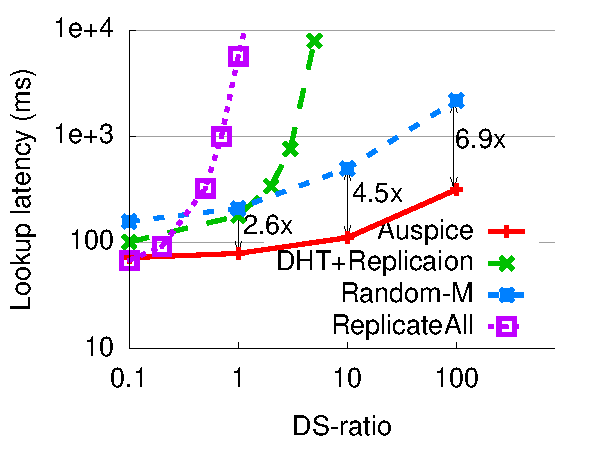
\includegraphics[scale=0.5]{graph/medianlatencyVSnummobile.pdf}
\vspace{-0.1in}
\caption{[Simulator] \auspice\ gives greater latency gains over \staticthree\ as the number of device names increases in  the workload.}
\label{fig:varymobile}
\end{figure}


\textbf{Ratio of device names to service names:} This experiment evaluates schemes for workloads with different ratios of device names to service names, called \emph{DS-ratio} for short.
We fix the number of service names to be 10K and vary the number of device names between 1000 to 1,000,000.
Figure \ref{fig:varymobile} presents our results.
\replicateall\  saturates server capacity for a workload with  DS-ratio = 1 due to high update costs. 
\auspice\  supports workloads with DS-ratio up to 100  as it minimizes the update cost for device names. 
Due to its locality-aware design, \auspice\ has  2.6$\times$, 4.5$\times$ and 6.9$\times$ lower latency than \staticthree\ when DS-ratios are 1, 10 and 100 respectively. 

 \codons's latency increases more sharply than \auspice\ and \staticthree\  on increasing the number of device names.  
\codons\ creates  a greater number of replicas for device names than \auspice\ and \staticthree, which increases update cost and, as a result, the lookup latency for \codons.
For example, for a workload with DS-ratio = 2  and an average hop count of 2.0, \codons\ creates an average of 24 replicas/name compared to three replicas/name for \staticthree. We experimented with average hop-count values as high as 10, but the number of replicas did not reduce further.
}



\eat{
\subsubsection{Scalability analysis}

Figure \ref{fig:scalability} evaluates the scalability of \auspice. In this experiment, we increase the number of name servers from 100 and 100,000, while keeping the total system capacity to be constant. The figure shows that \auspice\ is able to achieve the lowest latency while at the same time scales well to increasing number of servers. In contrast, \replicateall\ and \codons\ have poor scalability performance and saturate quickly.

To illustrate the scalability benefits of \auspice, consider a back of the envelope calculation based on the maintenance cost (\$\$) and network bandwidth needed for record update. Assume the number of servers increases by one order of magnitude (e.g., from 100 to 1000) while the total system capacity remains the same. Then \codons\ and  \replicateall\ will incur the same order of magnitude increase in terms of server maintenance cost and update bandwidth, because they replicate names at one order of magnitude more replicas and simply ignore the capacity constraint of the whole system. However, \auspice\ replicate names making sure that the aggregate system load is below a threshold of the capacity(refer \S 3.2.1), therefore it does incur additional maintenance cost and update bandwidth.

\begin{figure}
\centering
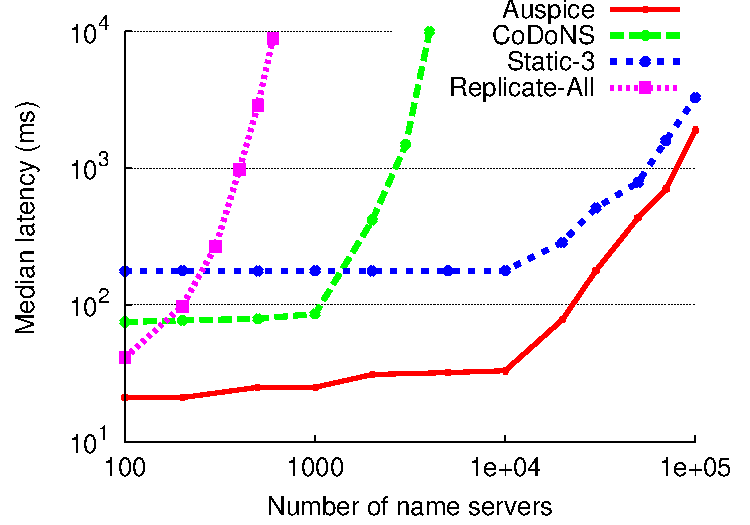
\includegraphics[scale=0.5]{graph/medianlatencyVSnumns.pdf}
\vspace{-0.1in}
\caption{[Simulator] \auspice\ scales well to increasing number of name servers. }
\label{fig:scalability}
\vspace{-0.1in}
\end{figure}

}


\eat{
\section{Limitations}
\auspice\ presented so far have outperformed existing DHT-based and managed DNS services in many aspects, however, there are limitations to its design and evaluation. 
First, we used a synthetic workload for mobile names and varied several parameters (e.g, ratio of service to device names, read to write rates, geo-locality) in the workload for a more comprehensive evaluation. However, the synthetic workload may not generalize to other patterns of mobile name changes and it is unclear the benefits of \auspice\ in a broader scope.
}
%Second, we show that  \auspice\ handles mid-session mobility well in our evaluation (TBD section) while leaving open the comparison against other alternatives, because it is not clear how existing network-layer approaches handle mobility. 
%Third, we use Paxos to ensure system consistency, but the cost of maintaining Paxos instances may be big. 
%Finally, \auspice\ may be vulnerable to malicious attackers without a robust security mechanism  and we leave it to the future work.

%\textbf{Comparison to DMap:}



%\vsp
%\subsubsection{Other results}
%\label{sec:other}


%We summarize a few other simulation-based results here with details deferred to a techreport \cite{techreport}.

%\textbf{Mid-session mobility:} We have shown connection migration across networks using MSocket when a single end-point (client) switches from a Wi-Fi to a 4G connection during an ongoing file transfer over TCP. The migration successfully completes within three round trip times using bilateral client-server negotiation.

%\textbf{Simulator validation:} We compare the results from our simulator to a PlanetLab experiment for  replication schemes in Section \\ref{sec:schemes}. The median latencies for all schemes in the simulator are within 8\% of that on PlanetLab. The 95\%-ile latencies are higher on PlanetLab experiments than in the simulator due to unpredictable wide area latencies and server processing delays.

%optimization formulation described in the techreport \cite{techreport}. \optimal\ decides both  replica placement and request redirection to minimize the sum of  network and server latency. The inputs  are  %We evaluate this scheme only in simulation, as it is not implemented in the prototype.

\eat{
\textbf{Optimal:} We have compared \auspice\ to \optimal\ based on an optimization formulation of the placement problem \cite{techreport}. 
\optimal\ takes as input  the set of names, their request geo-distribution, the capacity of name servers, network latency between local name servers and name servers, and a load-vs-response-time curve at each name server, and computes replica placement so as to minimize the sum of  network and server latency.
%In Figure \ref{fig:optimal}, we present the ratio of latency of \auspice\ to \optimal\  from this experiment. 
For a similar workload as in Section \\ref{sec:lookup},  we find that the latency for \auspice\ is between 1.1$\times$-2.1$\times$ of the \optimal\  across all load levels. \optimal\  performs better as it can globally optimize server resource allocation across all names, but \auspice\ uses a decentralized placement algorithm to independently decide replica placement for each name. 
In ongoing work, we are evaluating \optimal\  using the testbed; this is nontrivial partly because \optimal\ must know the exact load-vs-response time behavior, which is not always stationary or easy to measure, so we conjecture that the clean simulator environment overestimates the benefits of \optimal.
}

%\textbf{Workload sensitivity analysis:} We perform a sensitivity analysis of the workload parameters for device names using our simulator. (1) Geo-locality: \auspice\ gives better latencies as the geo-locality in the workload increases. For a completely random geo-distribution of requests, \auspice\ still outperforms \staticthree\ and \codons\ by 2$\times$ and $2.5\times$ respectively  as it maximizes the number of replicas under available server resources and redirects to the closest replica.  (2) Lookup-to-update ratio: \auspice\ gives better latencies than other replication schemes for lookup-to-update ratios both $>$ 1 and $<$ 1, instead of the default value of 1 used in earlier experiments. For a lookup-to-update ratio of 10, Auspice has 2.9$\times$ lower latency than Static-3.  

%(3) Service names to device names ratio: 

% Can be removed
%\textbf{Analysis of \auspice\ design:} We study variants of \auspice's design and show that locality-awareness in the placement of replicas and redirecting to a replica based on both network and server load-induced latency are two major factors that reduces lookup latency for \auspice\ in the PlanetLab experiments  (Section \\ref{sec:lowload}).

%\textbf{Comparison to locality-aware DHT:} We compare \auspice\ to a locality-aware DHT design, SkipNet. SkipNet assumes a hierarchical namespace, but in our workload consisting of flat names, gives  lower latencies than other DNS alternatives. 

%\textbf{TTL-value selection:} \auspice\ internally uses active replication, but does allow TTL-based caching at local name servers and clients. What TTL should names use? TTL-based caching means that \verb+connect(name,port)+ calls from end-hosts can occasionally time out because the destination \verb+name+ has moved. In this case, end-hosts must send a refresh query to \auspice\ and attempt to reconnect. The overall time-to-connect to a name depends on the name's update rate, lookup rate, and the TTL. We have developed a simple analytical model to calculate the optimal TTL based on these three values \cite{techreport} to serve as a recommendation to name owners\tbd{Do we have the expression? Without an expression, this seems content-free.}.

%We develop a analytical model to calculate the optimal TTL for a name at a cache that minimizes the connection-setup delay to the name. The optimal TTL is determined based on  lookup rate of a name at the cache and its update rate, and values of connection-setup delay in case of a cache hit, a cache miss, and a stale response from cache.  Simulations show that connection delays with the optimal TTL computed by our model gives a connection setup delay that is within 10\% of the minimum delay achievable.

